\documentclass[twoside]{article}

%\usepackage{aistats2020}
% If your paper is accepted, change the options for the package
% aistats2020 as follows:
%
\usepackage[accepted]{aistats2020}
%
% This option will print headings for the title of your paper and
% headings for the authors names, plus a copyright note at the end of
% the first column of the first page.

% If you set papersize explicitly, activate the following three lines:
%\special{papersize = 8.5in, 11in}
%\setlength{\pdfpageheight}{11in}
%\setlength{\pdfpagewidth}{8.5in}

% If you use natbib package, activate the following three lines:
\usepackage[round]{natbib}
\renewcommand{\bibname}{References}
\renewcommand{\bibsection}{\subsubsection*{\bibname}}

% If you use BibTeX in apalike style, activate the following line:
\bibliographystyle{apalike}

% graphics
\usepackage{float}
\usepackage{graphicx}

% math and stuff
\usepackage{amssymb}
\usepackage{amsmath}
\usepackage{amsthm}
\usepackage{algorithm}
\usepackage{algorithmicx}
\usepackage{algpseudocode}
%\newcommand{\disc}{\mathrm{disc}}
%\newcommand{\cont}{\mathrm{cont}}
%\newcommand{\tr}{\mathtt{tr}}
%\newcommand{\model}{\mathcal{P}}
%\newcommand{\proposal}{\mathcal{Q}}
\newtheorem{theorem}{Theorem}[section]
\newtheorem{corollary}{Corollary}[theorem]
\newtheorem{lemma}[theorem]{Lemma}

\begin{document}

% If your paper is accepted and the title of your paper is very long,
% the style will print as headings an error message. Use the following
% command to supply a shorter title of your paper so that it can be
% used as headings.
%
%\runningtitle{I use this title instead because the last one was very long}

% If your paper is accepted and the number of authors is large, the
% style will print as headings an error message. Use the following
% command to supply a shorter version of the authors names so that
% they can be used as headings (for example, use only the surnames)
%
%\runningauthor{Surname 1, Surname 2, Surname 3, ...., Surname n}

\twocolumn[

\aistatstitle{Automated Involutive MCMC}

\aistatsauthor{ Marco Cusumano-Towner \And Alexander K. Lew \And Vikash K. Mansinghka }

\aistatsaddress{ Massachusetts Institute of Technology } ]

\begin{abstract}
Involutive MCMC is a unifying framework for MCMC that encompasses many standard
and recent MCMC algorithms from the literature, from reversible jump MCMC to
Hamiltonian Monte Carlo to kernels based on deep neural networks. The key idea
in involutive MCMC is that a combination of (i) an auxiliary probability
distribution and (ii) an involution on the extended state space that includes
the model latent variables and the auxiliary variables results in MCMC kernels
that satisfy detailed balance with respect to the target distribution. The
involutive MCMC framework is appealing for its simplicity and generality, and
promises to be a useful conceptual and mathematical tool for exploring the
design space of MCMC kernels. However, like other Monte Carlo samplers,
implementing involutive samplers is time consuming and error prone. This paper
describes a technique for automatically generating the implementation of
involutive MCMC samplers from two probabilistic programs that define the target
distribution and the auxiliary probability distribution respectively, and a
differentiable program that defines the involution. The technique also detects
common conceptual and programming errors that arise when designing and
specifying involutive MCMC algorithms. This paper describes the support for
involutive MCMC in the Gen probabilistic system that uses this technique, and
shows involutive samplers specified using Gen's high-level probabilistic and
differentiable programming languages.
\end{abstract}

\section{INTRODUCTION}

%This is the best paper~\citep{cusumano2019gen}.

\subsection{Second Level Heading}

\subsubsection{Third Level Heading}

\paragraph{Fourth Level Heading}

\section{BACKGROUND AND RELATED WORK}

\subsection{Traces}

\begin{figure*}[ht]
    \centering
    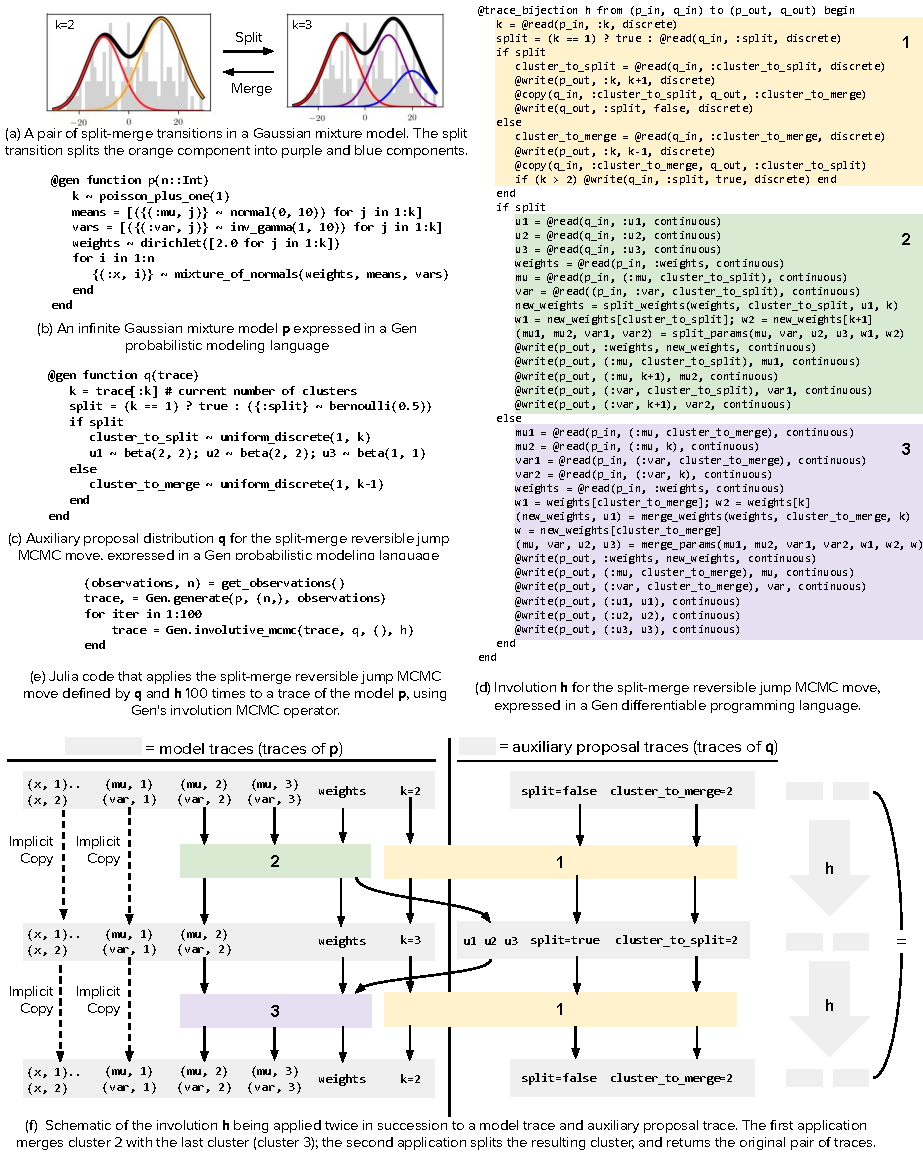
\includegraphics[width=\textwidth]{figures/mixture.pdf}
    \caption{
Example of reversible jump MCMC~\citep{green1995reversible} implemented using involutive MCMC in Gen.
The example implements a `split-merge move' in a infinite Gaussian mixture model~\citep{richardson1997bayesian} using three Gen programs:
(1) a probabilistic program $\mathtt{p}$ encoding the generative model (shown in b),
(2) a probabilistic program $\mathtt{q}$ encoding an auxiliary probability distribution (shown in c),
and (3) a differentiable program $\mathtt{h}$ that encodes an involution on the space of pairs of traces of $\mathtt{p}$ and $\mathtt{q}$ (shown in d).
Gen's involutive MCMC operator (shown in e) automatically computes the acceptance probability.
}
    \label{fig:mixture}
\end{figure*}

\begin{figure*}[ht]
    \centering
    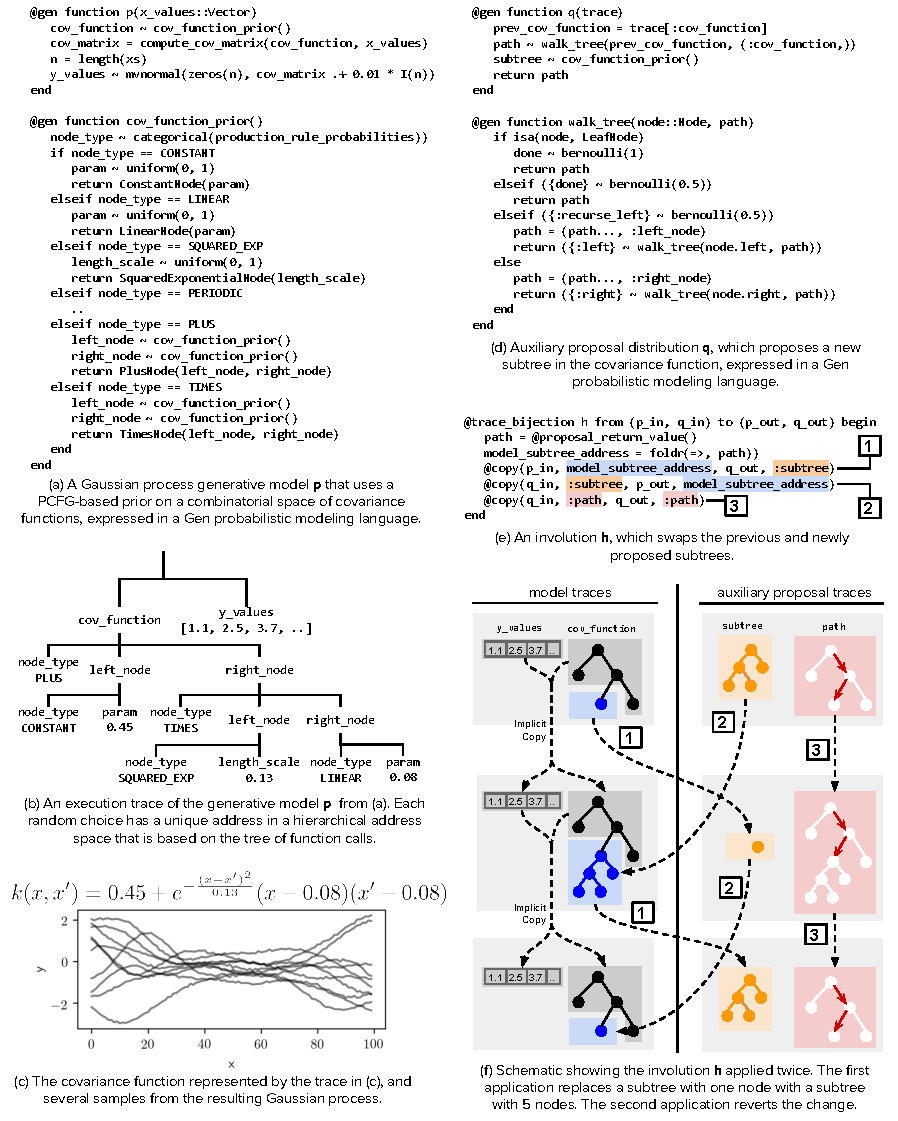
\includegraphics[width=\textwidth]{figures/structure-learning.pdf}
    \caption{
A mixture kernel implemented using involutive MCMC in Gen, applied to infer the covariance function of a Gaussian process.
The prior on covariance functions is based on a probabilistic context-free grammar.
Each component kernel in the mixture replaces a subtree of the covariance function parse tree with a new subtree.
The mixture kernel chooses a random subtree to replace via a random walk on the parse tree.
The mixture kernel is composed from three Gen programs:
(1) a probabilistic program $\mathtt{p}$ encoding the generative model (shown in a),
(2) a probabilistic program $\mathtt{q}$ encoding an auxiliary probability distribution (shown in b), and
(3) a differentiable program $\mathtt{h}$ that encodes an involution (shown in d).
}
    \label{fig:structure-learning}
\end{figure*}

\section{INVOLUTIVE MCMC}
Let $p$ denote the target probability density with respect to some $\sigma$-finite measure $\mu_X$ on a set $X$.
For each $x$ such that $p(x) > 0$, let $q_x$ denote a probability density with respect to some $\sigma$-finite measure $\mu_U$ on a set $U$.
Let $\mu := \mu_X \times \mu_U$ denote the product measure on the space $X \times U$, and let $\pi(x, u) := p(x) q_x(u)$ and $Z := \{(x, u) : \pi(x, u) > 0\}$.
Let $f : Z \to Z$ denote an involution ($f^{-1} = f$) such that the pushforward of $\mu$ under $f$, denoted $\mu \circ f^{-1}$, is absolutely continuous with respect to $\mu$, with Radon-Nikodym derivative $d (\mu \circ f^{-1}) / d\mu : Z \to [0, \infty)$.

\begin{algorithm}[h]
\begin{algorithmic}
\Procedure{involutive-mcmc-move}{$p$, $q$, $f$, $x$}
    \State $u \sim q(\cdot; x)$ \Comment{Sample auxiliary variables}
    \State $(x', u') \gets f(x, u)$ \Comment{Apply involution}
    %\State $\alpha \gets
        %\frac{p(x') q(u'; x')}{p(x) q(u; x)} \left| \left[ \frac{\partial h(u, t)}{\partial (u, t)} \right] \right|$
    % TODO or should we show the Radon-Nikodym derivative?
    \State $\alpha \gets
        \displaystyle \frac{p(x') q_{x'}(u')}{p(x) q_{x}(u)} \left( \frac{d (\mu \circ f^{-1})}{d \mu} (x, u)\right)^{-1}$
    % TODO check it
    \State $r \sim \mathrm{Uniform}(0, 1)$
    \State \algorithmicif \, $r \le \alpha$ \algorithmicthen \, \Return $x'$ \algorithmicelse \, \Return $x$ 
\EndProcedure
\end{algorithmic}
\caption{Involutive MCMC}
\label{alg:involutive-mcmc}
\end{algorithm}

\begin{lemma}\label{lemma:involution-detailed-balance} % TODO cite
For $p$, $q$, and $f$ satisfying the properties above, let $k'$ denote the following transition kernel on $Z$:
\[
k'_z(A) := [f(z) \in A] \alpha(z) + [z \in A](1 - \alpha(z))
\]
The transition kernel $k'$ on $Z$ defined by the involution $f$ satisfies detailed balance with respect to $\pi$:
\[
\int_B k'_z(A) \pi(dz) = \int_A k'_z(B) \pi(dz) \mbox{ for all } A, B \in \Sigma_Z
\]
And in particular it is stationary with respect to $\pi$:
\[
\int_Z k'_z(A) \pi(dz) = \pi(A) \mbox{ for all } A \in \Sigma_Z
\]
\end{lemma}
\begin{proof}
\end{proof}

\begin{theorem}\label{theorem:stationarity}
The transition kernel $k$ on $X$ defined by Algorithm~\ref{alg:involutive-mcmc} for valid $p$, $q$, and $f$:
\[
k_x(A) := \int_U k'_{x,u}(A \times U) q_x(u) \mu_U(du) \;\; \mbox{for all} \;\; A \in \Sigma_X, x \in X
\]
is stationary with respect to $p$.
\end{theorem}
\begin{proof}
By Lemma~\citep{lemma:involution-detailed-balance}, the transition kernel $k'$ is stationary with respect to $\pi$:
\[
%\int_B k'_{z}(B) \pi(z) \mu(dz) = \pi(B) \mbox{ for all } z \in X \times U, B \in \Sigma_Z
\]
It suffices to show that
\begin{align*}
\int_X k_x(A) p(x) \mu_X(dx) &= p(A) \mbox{ for all } A \in \Sigma_X\\
\int_X \left( \int_U k'_{x,u}(A \times U) q_x(u) \mu_U(du) \right) p(x) \mu_X(dx) &= p(A)\\
\int_{X \times U} k'_{x,u}(A \times U) q_x(u) p(x) \mu(dz) &= p(A)
\end{align*}
By Lemma~\citep{lemma:involution-detailed-balance}, setting $B := X \times U$, the left-hand-side is:
\[
\pi(X \times U) = \int_X \int_U p(x) q_x(u) \mu(
\]
\end{proof}
\paragraph{Detailed balance of the involution}
%Let $q_

\paragraph{Stationarity}

\paragraph{Conditional distribution and observations fixed}

% TODO PyTorch implementation??

\section{AUTOMATIC ACCEPTANCE PROBABILITY CALCULATION}

\subsection{Exploiting Jacobian Sparsity}

% TODO can only show this for a special case -- discrete involution + continuous?, or some more general case?

% TODO show an performance table of moves per second with and without the sparsity reduction (?)

\section{A DYNAMIC CHECK FOR DETECTING BUGS}

% TODO show an example of the type of bug it can detect (an edge case?)

\section{EXAMPLES}


\subsubsection*{Acknowledgements}
All acknowledgments go at the end of the paper, including thanks to reviewers who gave useful comments, to colleagues who contributed to the ideas, and to funding agencies and corporate sponsors that provided financial support.

\bibliography{references} 

\clearpage
\onecolumn
\section*{APPENDIX}

\subsection{Distributions on traces}
Define target density $\pi$ (XXX below it is called $p$, fix this) on the joint space $X \times U$, where $X$ are traces of the model and $X$ are traces of the proposal, in terms of the density $p(x)$ and the family of densities $q_x(u)$ as $\pi(x, u) := p(x) q_u(x)$.

% TODO rename the joint target density to \pi below
We want to show stationarity with respect to $\pi$, using stationarity of the involution with respect to the joint density (below).
\begin{equation}
\int_X p(x) \ell_x(A) \mu(dx) = p(A) \mbox{ for all } A \in \Sigma
\end{equation}
where $\ell_x(A)$ is the probability of transitioning into set $A$ from $x$, and is given by:
\begin{equation}
\ell_x(A) := \int_U k_{(x, u)}(A \times U) \mu(du)
\end{equation}
where $k_{(x, u)}$ is the measure on $X \times U$ that is induced by applying the involution $h$ to the state $(x, u)$.
% TODO checkme


\subsection{Stationarity of the involution with respect to joint density}
Let $(Z, \Sigma, \mu)$ be a measure space of pairs of traces of the model and proposal, where $\mu$ is $\sigma$-finite.
Consider a $\mu$-measurable function $h : Z \to Z$ that is an involution ($h(h(z)) = z$) and let $\mu \circ h^{-1}$ denote the pushforward of $\mu$ under $h$, such that $\mu \circ h^{-1}$ is $\sigma$-finite and such that $\mu \circ h^{-1}$ is absolutely continuous with respect to $\mu$.
% TODO can we simplify the conditions, using the fact that h is an involution?
Then, the Radon-Nikodym derivative exists, and is denoted $(d (\mu \circ h^{-1}) / d \mu)(z)$.

The goal is to prove stationarity with respect to the measure defined by density $p(z)$ with respect to $\mu$.
The move starts with state $z \in Z$, applies the involution $h$, and then accepts (returns $h(z)$) with probability $\alpha(z)$ and otherwise returns $z$.
Let $k_{z}$ denote the measure on new states induced by the involution $h$ and the previous state $z$:
\begin{equation}
k_{z}(A) = [h(z) \in A] \alpha(z) + [z \in A] (1 - \alpha(z))
\end{equation}
The stationarity condition is:
\begin{equation}
\int_Z p(z) k_{z}(A) \mu(dz) = p(A) = \int_Z p(z) [z \in A] \mu(dz) \mbox{ for all } A \in \Sigma
\end{equation}
Substituting in the definition of $k_z(A)$ and simplifying gives:
\begin{equation} \label{eq:stationarity-requirement}
\int_Z p(z) [h(z) \in A] \alpha(z) \mu(dz) = \int_Z p(z) [z \in A] \alpha(z) \mu(dz) \mbox{ for all } A \in \Sigma
\end{equation}
Note that for a $\mu$-measurable function $g$ such that $g \circ h$ is integrable with respect to $\mu$:
\begin{equation} \label{eq:pushforward}
\int_Z g(h(z)) \mu(dz) = \int_Z g(z) (\mu \circ h^{-1})(dz) = \int_Z g(z) \left( \frac{d (\mu \circ h^{-1})}{d \mu}(z) \right) \mu(dz)
\end{equation}
For $g(z) := p(h(z)) [z \in A] \alpha(h(z))$ we have $g(h(z)) = p(z) [h(z) \in A] \alpha(z)$, which is the integrand of the left-hand-side of Equation~(\ref{eq:stationarity-requirement}).
Applying Equation~(\ref{eq:pushforward}) to the left-hand side of Equation~(\ref{eq:stationarity-requirement}) gives:
\begin{equation}
\int_Z p(z) [h(z) \in A] \alpha(z) \mu(dz) = \int_Z g(z) \left( \frac{d (\mu \circ h^{-1})}{d \mu}(z) \right) \mu(dz) = \int_Z p(h(z)) [z \in A] \alpha(h(z)) \left( \frac{d (\mu \circ h^{-1})}{d \mu}(z) \right) \mu(dz)
\end{equation}
Equating this with the right-hand side of Equation~(\ref{eq:stationarity-requirement}) gives the following sufficient condition for stationarity:
\begin{equation}
\int_Z p(h(z)) [z \in A] \alpha(h(z)) \left( \frac{d (\mu \circ h^{-1})}{d \mu}(z) \right) \mu(dz) = \int_Z p(z) [z \in A] \mu(dz) \mbox{ for all } A \in \Sigma
\end{equation}
It therefore suffices to find $\alpha$ such that:
\begin{equation}
p(h(z)) [z \in A] \alpha(h(z)) \left( \frac{d (\mu \circ h^{-1})}{d \mu}(z) \right) = p(z) [z \in A] \alpha(z) \mbox{ for all } z \in Z
\end{equation}
The following choice of $\alpha$ suffices:
\begin{equation}
\alpha(z) = \min\left\{ 1, \frac{p(h(z))}{p(z)} \left( \frac{d (\mu \circ h^{-1})}{d \mu}(z) \right) \right\}
\end{equation}

All requirements:
\begin{enumerate}
\item $\mu$ is $\sigma$-finite
\item $h$ is $\mu$-measurable
\item $h$ is an involution
\item the pushforward $\mu \circ h^{-1}$ is $\sigma$-finite
\item the pushforward $\mu \circ h^{-1}$ is absolutely continuous with respect to $\mu$
\item the function $g(z) := p(h(z)) [z \in A] \alpha(h(z))$ is $\mu$-measurable for all $A \in \Sigma$
\item the function $(g \circ h)(z) = p(z) [h(z) \in A] \alpha(z)$ is integrable with respect to $\mu$ for all $A \in \Sigma$
\end{enumerate}

\paragraph{Characterizing the pushforward $\mu \circ h^{-1}$ for involution $h$}
Can we guarantee that it is $\sigma$-finite or absolutely continuous with respect to $\mu$?
Are there simpler sufficient conditions we can give?
$(\mu \circ h^{-1})$ is $\sigma$-finite if $Z$ is the countable union of $(mu \circ h^{-1})$-measurable sets with finite measure.

$\sigma$-finite means 

\section{Detailed balance}

Can we employ Theorem 2 of Tierney 1998? How does this relate to how the algorithm is described.
Tierney already employs it for the involution-based move for the joint space of model and proposal traces (see page 4, bullet point 2 'deterministic proposals').
But employing it for the composite move that includes the proposal and involution is more complex.
The elements are:
\begin{enumerate}
\item $x, y \in X$ and $(X, \Sigma_X, \mu_X)$, where $x$ are traces of the model, and $\pi(x)$ is the model (target) density.
\item $u \in U$ and $(U, \Sigma_U, \mu_U)$, where $u$ are traces of the proposal and $q_{x}(u)$ is the proposal density.
\item An involution $h : X \times U \to X \times U$ (properly restricted to the support of $\pi(x) q_{x}(u)$.
\end{enumerate}
We want to provide a detailed balance result on $(X, \Sigma_X, \mu_X)$, proving detailed balance with respect to $\pi(x)$.
Tierney's proposal kernel is defined by a family of measures $Q_{x} : \Sigma_X \to [0, \infty)$.
In our case, this is:
\[
Q_{x}(A) := \int_U [h(x, u)_1 \in A] q_{x}(du) = \int_U [h(x, u)_1 \in A] q_{x}(u) \mu_U(du)
\]
Tierney's transition kernel with acceptance probability $\alpha(x \to y)$ is defined by a family of measures $P_x : \Sigma_X \to [0, \infty)$ (Equation 1 of Tierney):
\[
P_x(A) = \int_A \alpha(x \to y) Q_x(dy) + [x \in A] \int_X (1 - \alpha(x \to y)) Q_x(dy) \mbox{ for } A \in \Sigma_X
\]
Detailed balance (Tierney equation 2) is expressed as an equality between two measures on $X \times X$, denoted $(\pi P)_{\to}$ and $(\pi P)_{\gets}$.
\[
(\pi P)_{\to}(A, B) = (\pi P)_{\gets}(A, B)
\]
where
\[
(\pi P)_{\to}(A, B) := \int_A \left( \int_B P_x(dy) \right) \pi(dx)
\]
and
\[
(\pi P)_{\gets}(A, B) := \int_B \left( \int_A P_x(dy) \right) \pi(dx)
\]
Tierney Proposition 1 relies on a $\sigma$-finite measure $\mu$ on the product space $(X \times X, \Sigma_X \times \Sigma_X$), which is constructed as
the measure induced by first sampling $x$ according to $\pi$ and then sampling $y$ according to the proposal $Q_x$:
\[
\mu(A, B) := \int_A \left( \int_B Q_x(dy) \right) \pi(dx) \;\;\; \mu^T(A, B) := \mu(B, A)
\]
In our case, this is:
\[
\mu(A, B) := \int_A \left( \int_U [h(x, u)_1 \in B] q_{x}(du) \right) \pi(dx) = \int_A \left( \int_U [h(x, u) \in B \times U] q_{x}(du) \right) \pi(dx)
\]
\paragraph{Show that $\mu$ is $\sigma$-finite (a requirement for Tierney Proposition 1)}
$X \times X$ needs to be the countable union of measurable sets with finite measure $\mu(X \times X)$.
It should build on the fact that $\pi$ and $q_x$ are $\sigma$-finite.
%Can we use the fact that the composition of two $\sigma$-finite kernels is itself $\sigma$-finite (where the first kernel is $\pi$ and has a trivial index space)?
%Apparently 
%If so, then it would suffice to show that $Q$ is a $\sigma$-finite kernel, which is true if all $Q_x$ are $\sigma$-finite measures.

\paragraph{Characterize $R$, and $\mu_R$ is the restriction of $\mu$ to $R$, and $\mu_R^T$ is as above}


\paragraph{Characterize the following Radon-Nikodym derivative of $\mu_R$ with respect to $\mu_R^T$}
\[
r(x, y) = \frac{d\mu_R}{d\mu_R^T}(x, y)
\]
We need to show that:
\begin{enumerate}
\item $\alpha$ is $\mu$-almost everywhere zero on $R^c$
\item $\alpha(x, y) r(x, y) = \alpha(y, x)$
\end{enumerate}
Then, according to Tierney Proposition 1, there exists a (unique up to null-sets) symmetric set $R \in \Sigma_X \times \Sigma_X$ such that $\mu$ and $\mu^T$ are mutually absolutely continuous.
%(TODO: constructing $R$ for our kernel is a key step).

\subsection{Special case of involution on discrete + diffeomorphism}

\section{Using Tierney's result for deterministic proposals}

\paragraph{Step 1: determine the acceptance ratio based on Tierney's involution construction}
(page 4 of Tierney 1998)
$T$ is the involution and $E$ is the joint space $X \times U$.
Define the measure $\pi'$ by $\pi'(A) = \pi(T^{-1}(A))$ for all $A \in \Sigma_X$
and let $\nu(dx) = \pi(dx) + \pi'(dx)$.
Let $h(x)$ be a density for $\pi(dx)$ with respect to $\nu(dx)$ (( TODO this is they key step )).

\paragraph{Step 2: prove stationarity for the end-to-end kernel}
Using stationarity of the involutive kernel, which derives from Step 1.

\section{Derivation of pushforward Radon-Nikodym derivative for special case}
TODO: Do some special case where it simplifies to a Jacobian determinant.
Maybe the case where the involution is composed of an involution on discrete part and a diffeomorphism on the continuous part.

\section{Proof of detailed balance for involution}
\citet{tierney1998note} gives a class of MCMC kernels based on involutions that satisfy detailed balance.
Specifically, given an involution $T : Z \to Z$, they denote the pushforward of $\pi$ under $T$ by $\pi'$:
$\pi'(A) := \pi(T^{-1}(A))$.
They let $\nu(A) := \pi(A) + \pi'(A)$.
They let $h(z)$ denote `a density for $\pi$ with respect to $\nu$'.
Then, they set:
\[
\alpha(x \to T(x)) \frac{h(x)}{h(T(x))} = \alpha(T(x) \to x)
\]
To use this result, it suffices to show that $h$ simplifes to the following, when $\pi$ and $\pi'$ are $\sigma$-finite and have densities with respect to the same reference measure $\mu$:
\[
\frac{h(z)}{h(T(z))}= \frac{\pi(z)}{\pi(T(z))} \left( \frac{d (\mu \circ T^{-1})}{d \mu} \right)^{-1}
\]
(note that $T$ is our $f$).
What is $h(z)$, the density of $\pi$ with respect to $\nu(A) := \pi(A) + \pi'(A)$?
Well, if $\pi$ and $\pi'$ have densities with respect to $\mu$, then so does $\nu$, and it is $\nu(z) = \pi(z) + \pi'(z)$.
Then, the density of $\pi$ with respect to $\nu$ is:
\[
h(z) = \frac{\pi(z)}{\nu(z)} = \frac{\pi(z)}{\pi(z) + \pi'(z)}
\]
It suffices to show that:
\[
\frac{h(z)}{h(T(z))} = \frac{\pi(z)}{\pi(T(z))} \frac{\pi(T(z)) + \pi'(T(z))}{\pi(z) + \pi'(z)}
= \frac{\pi(z)}{\pi(T(z))} \left( \frac{d (\mu \circ T^{-1})}{d \mu} \right)^{-1}
\]
It suffices to show that:
\[
\frac{\pi(T(z)) + \pi'(T(z))}{\pi(z) + \pi'(z)} = \left( \frac{d (\mu \circ T^{-1})}{d \mu} \right)^{-1}
\]
Let $a(z) = \pi(z) + \pi'(z)$, and note that $a$ is a density with respect to $\mu$.
Then, the ratio above is:
\[
\frac{\pi(T(z)) + \pi'(T(z))}{\pi(z) + \pi'(z)} = \frac{a(T(z))}{a(z)}
\]
Consider the measure $a$ on $Z$ and the pushforward measure $a \circ T^{-1}$ on $Z$.
It suffices to show that
\[ 
1 = \frac{d (a \circ T^{-1})}{d a} = \frac{a(T(z))}{a(z)} \left( \frac{d (\mu \circ T^{-1})}{d \mu} \right)
\]
$\frac{d (a \circ T^{-1})}{d a} = 1$ follows from the fact that $a$ and $a \circ T^{-1}$ are actually the same measure:
\begin{align}
a(B) &= \pi(B) + \pi'(B) = \pi(B) + \pi(T^{-1}(B))\\
(a \circ T^{-1})(B) &= \pi(T^{-1}(B)) + \pi(T{-1}(T^{-1}(B))) = \pi(T^{-1}(B)) + \pi(B)
\end{align}
Using the chain rule (TODO check this!):
\[
1 = \frac{d (a \circ T^{-1})}{d a}
=   \frac{d (a \circ T^{-1})}{d (\mu \circ T^{-1})}
    \frac{d (\mu \circ T^{-1})}{d \mu}
    \frac{d \mu}{d a}
= a(T(z))  \frac{d (\mu \circ T^{-1})}{d \mu} \frac{1}{a(z)}
\]
Note that $a$ is actually equivalent to Tierney's $\nu$.
The non-obvious part is the first factor:
\[
\frac{d (a \circ T^{-1})}{d (\mu \circ T^{-1})}(z) = \frac{d a}{d \mu} (T(z))
\]
TODO: prove me!

\section{Proof of stationarity for involution}
Stationarity follows from detailed balance by setting $B := Z$ in the detailed balance equation, and using $k'_z(Z) = \alpha(z) + (1 - \alpha(z)) =1$, so the right-hand side simplifies to $\int_A \pi(dz) = \pi(A)$.

\section{Proof of stationarity for end-to-end kernel}
We are given that the involution is stationary with respect to (the measure induced by) $\pi(x, u) := p(x) q_x(u)$:
\[
\int_Z k'_z(A) \pi(z) \mu(dz) = \pi(A) \mbox{ for all } A \in \Sigma_Z
\]
It suffices to show that the end-to-end kernel $k$ is stationary with respect to (the measure induced by) $p(x)$:
\[
\int_X k_x(A) p(x) \mu_X(dx) = p(A) \mbox{ for all } A \in \Sigma_X
\]
The kernel $k$ on $X$ defined by Algorithm~\ref{alg:involutive-mcmc} for valid $p$, $q$, and $f$:
\[
k_x(A) := \int_U k'_{x,u}(A \times U) q_x(u) \mu_U(du) \;\; \mbox{for all} \;\; A \in \Sigma_X, x \in X
\]
is stationary with respect to $p$.
\begin{align*}
    \int_X k_x(A) p(x) \mu_X(dx) &= p(A) \mbox{ for all } A \in \Sigma_X\\
    \int_X \left( \int_U k'_{x,u}(A \times U) q_x(u) \mu_U(du) \right) p(x) \mu_X(dx) &= p(A)\\
    \int_{X \times U} k'_{x,u}(A \times U) q_x(u) p(x) \mu(dz) &= p(A)\\
    \int_{X \times U} k'_{x,u}(A \times U) \pi(z) \mu(dz) &= p(A)\\
    \pi(A \times U) &= p(A)\\
    \int_{A \times U} q_x(u) p(x) \mu(dz) &= p(A)\\
    \int_A \left( \int_U q_x(u) \mu_U(du) \right) p(x) \mu_X(dx) &= p(A)\\
    \int_A p(x) \mu_X(dx) &= p(A)
\end{align*}
% TODO characterize the various assumptions that allow us to e.g. rearrange the order of integration, etc.

\end{document}
